\section{Technical Architecture}
\label{sec:architecture}

The technical architecture of Educational MicroSims represents a carefully balanced approach to creating interactive educational content that maximizes accessibility, maintainability, and generative AI compatibility. The architecture prioritizes web standards, responsive design principles, and educational transparency while minimizing technical complexity and deployment requirements.

The design decisions underlying the MicroSims architecture emerge from extensive analysis of educational technology deployment scenarios, ranging from individual student devices to institutional learning management systems. The architecture addresses the fundamental challenge of creating interactive content that functions reliably across diverse technical environments while remaining simple enough for educators and students to understand, modify, and extend.

\subsection{Technology Stack}

\begin{figure}[htbp]
\centering
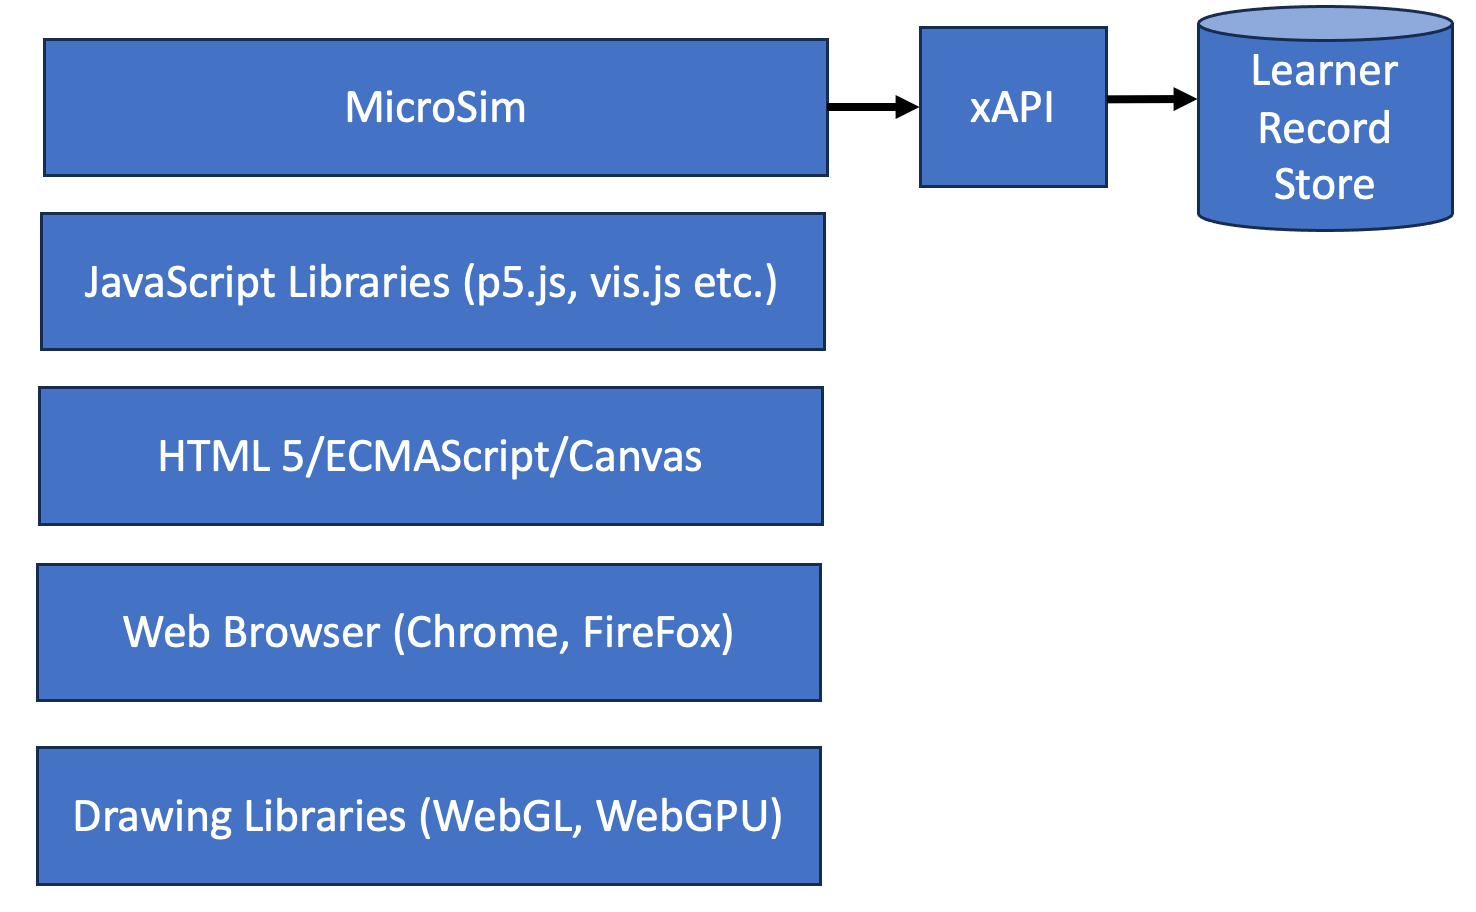
\includegraphics[width=0.6\textwidth]{figures/microsim-architecture.png}
\caption{MicroSims use a standardized web deployment architecture depicted as a series of layers. The foundation is built on HTML-5, JavaScript standards (ECMAScript), ensuring broad compatibility across browsers and devices. Modern browsers such as Chrome ane FireFox can leverage consistent low-level drawing libraries such as WebGL and WebGPU for fast rendering of complex 3D simulations. The p5.js library provides the core drawing and interaction capabilities, while the MicroSims framework extends p5.js with standardized patterns for responsive design, user interface management, and educational data collection. This layered architecture supports seamless embedding within iframe elements, enabling integration with diverse educational platforms while maintaining security and performance.  A MicroSIm can optionally generate xAPI JSON statements to report user interactions to learning record stores for integration with intelligent textbooks and learning analytics systems.  Analysis of student interaction data can be used to adaptively modify the simulation experience using reinforcement learning techniques.}
\label{fig:architecture}
\end{figure}

\subsubsection{p5.js Foundation}

The technical architecture of the MicroSims framework is built upon the p5.js creative coding library, selected for its educational transparency, extensive documentation, and gentle learning curve. p5.js provides a comprehensive set of drawing and interaction primitives while maintaining code readability that enables educators and students to understand and modify simulation logic. The framework extends p5.js capabilities with standardized patterns for responsive design, user interface management, and educational data collection.

The selection of p5.js as the foundational technology reflects several critical architectural requirements. First, p5.js prioritizes educational accessibility through its simplified syntax and comprehensive documentation ecosystem. Second, the library's focus on immediate visual feedback aligns perfectly with the pedagogical goals of interactive simulations. Third, p5.js maintains broad browser compatibility without requiring complex build processes or development toolchains, enabling direct deployment and modification in educational environments.

The architecture defines a modular structure where core simulation logic is separated from presentation and interaction layers. This separation enables simulations to be easily modified or extended without affecting the underlying educational model. The framework provides standardized templates for common simulation types, incorporating best practices for code organization, naming conventions, and documentation standards.

\subsubsection{MicroSim Rules Files}

A critical component of the MicroSims architecture is the comprehensive rules file system that enables generative AI systems to create consistent, high-quality educational simulations. These rules files codify the design patterns, layout conventions, and implementation standards that ensure uniformity across different AI-generated content while maintaining educational effectiveness.  Modern generative AI systems can utilize these rules files to produce MicroSims that adhere to established pedagogical and technical standards.  Examples of these rules are `skills` files that are mapped to specific content generation tasks.

The rules files define three primary layout types that accommodate different educational simulation requirements. Fixed layouts provide simple positioning for basic demonstrations, responsive width layouts adapt horizontally to container dimensions while maintaining fixed heights, and two-column layouts separate simulation visualization from data analysis components. Each layout type includes specific implementation patterns, variable naming conventions, and responsive behavior specifications.

The standardization extends to user interface design patterns, including consistent control placement, labeling conventions, and interaction feedback mechanisms. All interactive elements follow prescribed positioning relative to the drawing area, with sliders expanding to utilize available width and buttons maintaining consistent spacing and styling. The rules ensure that generated simulations include proper accessibility features, responsive behavior, and educational transparency.

Precise rules files are critical for efficient generation of MicroSims by large language models (LLMs).  By carefully structuring rules files only the relevant rules need to be brought into the context window of the LLM, allowing it to focus on the specific generation task without being overwhelmed by extraneous information.  This targeted approach enhances the quality and consistency of AI-generated simulations while reducing computational overhead.

\subsubsection{HTML5 Canvas and Cross-Platform Compatibility}

The MicroSim framework leverages HTML5 Canvas capabilities to provide rich interactive experiences while maintaining compatibility across diverse devices and platforms. Canvas-based rendering ensures consistent visual output across different browsers and operating systems, while HTML5 audio and video elements support multimedia integration when pedagogically appropriate. The architecture avoids features that require plugin installation or platform-specific implementations, ensuring universal accessibility.

Cross-platform compatibility is validated through systematic testing across major web browsers and mobile platforms. The framework includes performance optimization techniques that ensure smooth operation on lower-powered devices commonly found in educational environments, including older tablets and budget smartphones. Browser compatibility considerations include progressive enhancement strategies where advanced features degrade gracefully on older platforms while maintaining core functionality.

\subsection{Width-Responsive Design Implementation}

Width-responsive design represents the optimal architectural approach for Educational MicroSims, providing essential flexibility without unnecessary complexity. This design philosophy ensures that simulations automatically adjust their horizontal dimensions to match their container while maintaining a fixed height, creating an ideal balance between adaptability and predictability.  An example of a width-responsive rule is to place the title in the top of the canvas and centered at half the width of the canvas.  Using the proper textAlign setting in p5.js makes this easy to implement.

The width-responsive approach addresses critical educational deployment scenarios. In learning management systems, MicroSims fit within content columns of different widths without horizontal scrolling. On mobile devices, students can interact with simulations on phones and tablets with touch controls remaining accessible regardless of screen width. In classroom projection scenarios, teachers benefit from full utilization of projector width with larger controls and text for back-of-room visibility.

The technical implementation involves container detection, where the simulation reads the parent container's width on initialization, dynamic canvas creation with container width and fixed height, and proportional control positioning relative to canvas width. Resize event handling updates the layout when window dimensions change, while content scaling adjusts visual elements proportionally to width changes.

\subsection{Layout Architecture}

\subsubsection{Canvas Regions}

The MicroSims layout architecture follows a standardized structure that divides the canvas into distinct functional regions. This approach ensures visual consistency across different simulations while providing clear separation between interactive content and user controls.

\begin{lstlisting}[caption={Standard MicroSim Canvas Structure}]
// Canvas dimensions
let canvasWidth = 400;              // Initial width (responsive)
let drawHeight = 400;                // Simulation area height
let controlHeight = 50;              // Controls area height
let canvasHeight = drawHeight + controlHeight;
let margin = 25;                     // Margin for visual elements
let sliderLeftMargin = 105;          // Left margin for slider positioning
\end{lstlisting}

The drawing area occupies the upper portion of the canvas with an 'aliceblue' background, providing a visually distinct region for simulation content. The controls area below uses a white background and contains all interactive elements including sliders, buttons, and labels. Both regions are outlined with a 1-pixel silver border to provide clear visual separation.

\subsubsection{Responsive Design Patterns}

The responsive design implementation utilizes container queries rather than viewport-based media queries, enabling MicroSims to adapt to their embedding context rather than the overall device screen. This architectural decision is particularly critical for educational applications where simulations may be embedded within learning management systems, digital textbooks, or other educational platforms with complex layout structures.

Container width adaptation is implemented through a standardized \texttt{updateCanvasSize()} function that recalculates layout parameters based on the detected container dimensions. This function triggers automatic repositioning of user interface elements, rescaling of text sizes within defined bounds, and adjustment of visualization areas to maintain optimal information density. The responsive system includes provisions for progressive disclosure, where complex simulations may hide or simplify certain interface elements on narrow displays.

\subsection{iframe Integration}

\subsubsection{Embedding Protocol}

A critical architectural requirement is seamless integration within iframe elements, enabling MicroSims to be embedded as single-line HTML elements within diverse educational platforms. The framework addresses common iframe integration challenges, including cross-origin communication, responsive sizing, and event handling. MicroSims are designed to function completely within iframe boundaries without requiring parent page modification or cross-frame scripting.

The iframe integration model supports both static and dynamic embedding scenarios. Static embedding involves simple HTML iframe tags with specified dimensions, suitable for content management systems and learning management platforms. Dynamic embedding utilizes JavaScript-based integration that can automatically adjust iframe dimensions based on content requirements and respond to container size changes.

The standardized embedding approach ensures that educational platforms can integrate MicroSims using minimal HTML code while maintaining full functionality. The responsive design automatically adapts to iframe dimensions, ensuring that simulations remain usable regardless of the embedding context or container constraints.

\subsubsection{Security Considerations}

Security considerations for iframe deployment include content security policy compliance and prevention of clickjacking vulnerabilities. The framework implements appropriate sandbox attributes and communication protocols that enable safe embedding while maintaining necessary functionality. Cross-origin resource sharing (CORS) policies are configured to support integration across different domain environments commonly found in educational technology ecosystems.

The architecture prioritizes client-side execution to minimize security risks associated with server-side processing or external data dependencies. All simulation logic executes within the browser environment, reducing potential attack vectors while ensuring that educational content remains accessible even in restrictive network environments.

Data privacy considerations are embedded throughout the architecture, with optional learning analytics integration designed to comply with educational privacy requirements. The framework provides clear separation between core simulation functionality and data collection capabilities, enabling institutions to deploy MicroSims in compliance with their specific privacy policies and regulatory requirements.

\subsubsection{Extended JavaScript Ecosystem}

While p5.js provides the foundational capabilities for most educational simulations, the MicroSims architecture accommodates integration with specialized JavaScript libraries for specific educational domains. For complex network visualizations, the framework supports integration with vis.js and vis-network.js libraries, enabling the creation of interactive graph-based educational content such as concept maps, social network analysis, and algorithm visualization.

Timeline-based educational content leverages vis-timeline.js for creating interactive historical timelines, project scheduling demonstrations, and temporal data analysis simulations. These integrations maintain the core MicroSims design principles while extending capabilities for specific educational requirements that exceed p5.js native functionality.

The extended ecosystem integration follows careful dependency management principles to preserve the lightweight characteristics essential for educational deployment. Each additional library is evaluated for educational necessity, performance impact, and compatibility with the core responsive design requirements.
